
\chapter{Menu Volumes}\label{volumes_chapter}
\minitoc 

\section{Edit first selected volume}
This option opens the "Edit first selected volume" window.
The "Edit first selected" window can also be opened by clicking on "
\includegraphics[scale=0.7]{images/06/objects/volume_edit.png}" (see Fig. \ref{edit_volume_window} p.\pageref{edit_volume_window}).



\begin{figure}
  \centering
  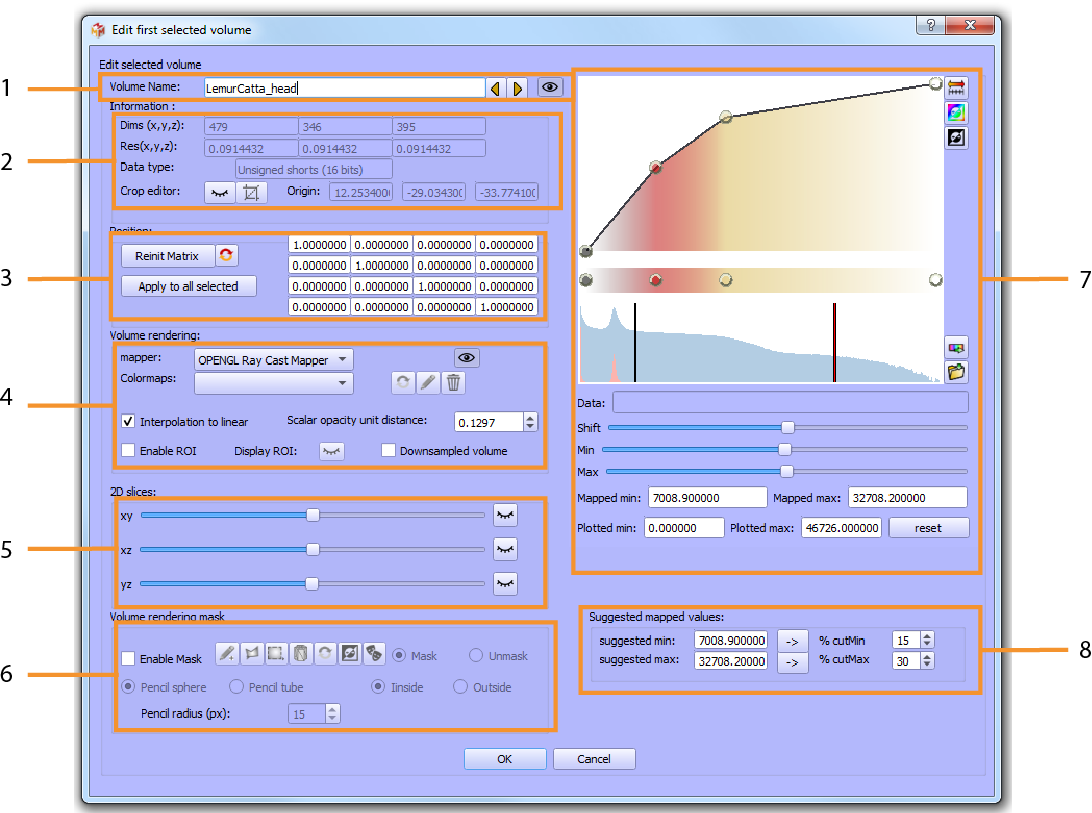
\includegraphics[scale=1]{images/14/edit_volume_window.png}
\caption{Edit first selected volume window. This window is divided in different subsections. \textbf{1)} Choose current volume to edit. Change volume name, browse through the different opened volume (arrows), and render or hide the currently activated volume rendering representation and/or 2D slices.  \textbf{2)} Information: dimensions, voxel size and data type of the currently selected volume. Crop editor: define crop region of the currently selected volume. \textbf{3)} Position matrix. Edit manually the position matrix, reinit matrix to identity, refresh matrix, and/or apply edited matrix to all selected volumes. \textbf{4)} Volume rendering. Choose mapper and colormap. Show or hide volume rendering representation. Show only a region of the currently selected volume (Enable ROI and display ROI toggles). \textbf{5)} 2D slices settings and visibility in xy, xz and yz planes. \textbf{6)} Volume rendering masking. Mask must be enabled first to activate the different masking tools : pencil sphere, pencil tube, free-form lasso, square lasso, use 3D surface to mask volume region, invert mask, and fill masked voxels.  \textbf{7)} Color map edition and histogram (orange: linear scale; blue: logarithmic scale). \textbf{8)} Map 3D volume using suggested min and suggested max values.}	
\label{edit_volume_window}
 \end{figure}

\subsection{Volume: name, selection and visibility}
Switching between all currently opened volume, editing their names can be performed in this section (see Fig.\ref{volume_name} p.\pageref{volume_name}).
\begin{figure}
  \centering
  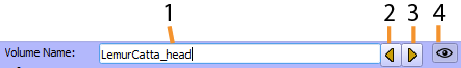
\includegraphics[scale=1]{images/14/volume_name2.png}
\caption{Volume: name, selection and visibility. \textbf{1)} View and/or change the name of the currently selected volume.  \textbf{2)} Select preceding volume.  \textbf{3)} Select next volume. \textbf{4)} make visible or hide all representations in the 3D window for the currently selected volume (volume rendering and/or 2D slices representations). }	
\label{volume_name}
 \end{figure}

\subsection{Information and crop editor}
Volume dimensions, resolution, data type and position in 3D space of the first voxel of the volume (origin) are available in this section (see Fig. \ref{volume_information} p.\pageref{volume_information}). The crop editor is also situated in this section. 
\begin{figure}
  \centering
  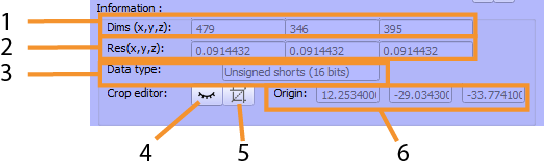
\includegraphics[scale=1]{images/14/volume_information2.png}
\caption{Volume information and crop editor. \textbf{1)} Number of voxels in X, Y and Z dimensions of currently selected volume.   \textbf{2)} Voxel resolution in X, Y and Z (scale: size unit most often expressed in mm). \textbf{3)} Data type (8 bits, 16 bits, 32 bits or 64 bits voxels).  \textbf{4)} Display / hide crop box. \textbf{5)} Apply crop box: restrict the dimensions of the currently opened volume to those of the crop box. \textbf{6)} Origin of the first voxel of currently selected volume in X,Y and Z. }	
\label{volume_information}
 \end{figure}


\subsection{Position}
Volume position matrix can be manually edited, reinitialized and refreshed inside this section (see Fig. \ref{volume_position} p. \pageref{volume_position}).
\begin{figure}
  \centering
  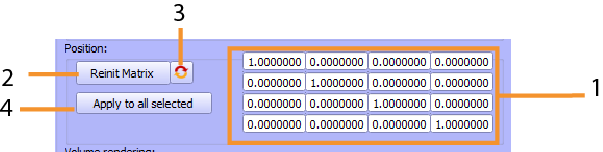
\includegraphics[scale=1]{images/14/volume_position2.png}
\caption{Volume position section. \textbf{1)} Position matrix.   \textbf{2)} Reset position matrix to identity. \textbf{3)} Refresh position matrix.  \textbf{4)} Apply position matrix to all selected volumes. }	
\label{volume_position}
 \end{figure}



\subsection{Volume rendering}
Volume rendering options are located in this section (see Fig. \ref{volume_rendering} p. \pageref{volume_rendering}).
\begin{figure}
  \centering
  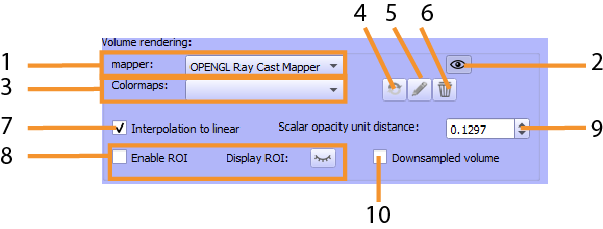
\includegraphics[scale=1]{images/14/volume_rendering2.png}
\caption{Volume rendering section. \textbf{1)} Chose mapper (note that "Smart Volume mapper" does not currently allow masks).   \textbf{2)} Display / hide volume rendering representation of currently selected volume. \textbf{3)} Change color map.  \textbf{4)} Reinitialize current colormap (only possible for default colormaps). \textbf{5)} edit current colormap name (only possible for user-defined colormaps.) \textbf{6)}delete current colormap (only possible for user-defined colormaps.) \textbf{7)} Activate/ deactivate linear interpolation rendering. \textbf{8)} Enable/ disable ROI clipping box, and display / hide clipping box boundaries and edition handles.  \textbf{9)} Change scalar opacity unit distance. \textbf{10)} Render a down-sampled version of the currently selected volume rather than the full volume (large volumes, e.g. > 1Gb datasets are often hard to render on standard graphics cards and may make your computer crash).  }	
\label{volume_rendering}
 \end{figure}

\subsection{2D slices}
Display of 2D slices inside the 3D main window is located in this section (see Fig. \ref{volume_2Dslices} p. \pageref{volume_2Dslices}).
\begin{figure}
  \centering
  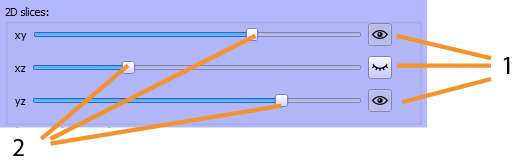
\includegraphics[scale=1]{images/14/volume_2Dslices2.png}
\caption{2D slices  \textbf{1)} Display / hide 2D slices in xy, xz and yz planes. \textbf{2)} Change slice number in xy, xz and yz planes.  }	
\label{volume_2Dslices}

 \end{figure}


\subsection{Volume rendering mask}\label{volume_rendering_masking}
Volume rendering masking tools are located in this section (see Fig. \ref{volume_masking} p. \pageref{volume_masking}). Note that when the Smart Volume Mapper is selected, masking tools become unavailable.
\begin{figure}
  \centering
  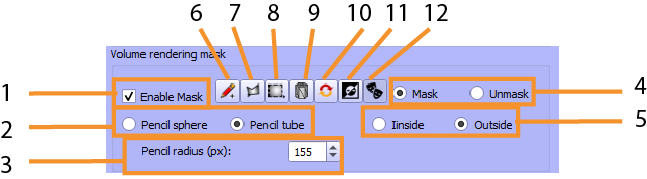
\includegraphics[scale=1]{images/14/volume_masking2.png}
\caption{Volume rendering mask.  \textbf{1)} Enable/disable mask tools. \textbf{2)} When using the pencil tool, choose between spherical shape and cylindric shape.  \textbf{3)} Define pencil radius in terms of screen pixels. Pencil radius can be interactively changed by keeping "T" pressed while rolling the middle mouse button.  \textbf{4)} Define whether voxels laying inside the selection should be masked or unmasked. \textbf{5)} Define whether selected voxels to mask/unmask laying inside or outside the selected region. \textbf{6)} Pencil selection tool. \textbf{7)} Lasso selection tool. \textbf{8)} Rectangular region selection tool.  \textbf{9)} 3D surface selection tool: use a 3D surface to define which region should be masked. \textbf{10)} Reinitialize mask. \textbf{11)} Invert mask. \textbf{12)} Harden transform mask. \textbf{13)} Import mask. \textbf{14)} Export mask.}	
\label{volume_masking}

 \end{figure}


\subsection{Color map edition}
Volume rendering color map edition controls tools are located in this section (see Fig. \ref{volume_colormap} p. \pageref{volume_colormap}). 
\begin{figure}
  \centering
  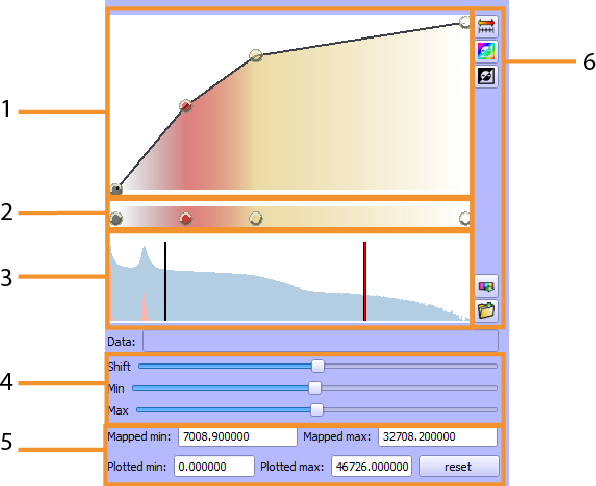
\includegraphics[scale=1]{images/14/volume_colormap2.png}
\caption{Volume rendering colormap control section. \textbf{1)} Opacity control points of the active color map (move these points to change opacity). \textbf{2)} Color control points of the active color map (double click on each point to edit the color). \textbf{3)} Histogram of currently selected volume. Orange: conventional histogram. Blue: logarithmic-scaled histogram. The 2 vertical bars indicate the min and max display range of the colormap.  \textbf{4)} Shift color map display range, or change min and max display range.\textbf{5)} Edit manually mapped min or max value. Edit manually histogram plotted min or max. \textbf{6)} From top to down. a: set range to min and max. b: reverse color control points. c: reverse opacity control points. d: Export colormap to file. e: Save colormap to presets = duplicate current active color map and create a new custom color map.}	
\label{volume_colormap}
 \end{figure}

\subsection{Suggested mapped values}
You may decide to reset min and max of the color map based on suggested values. These suggested min and max values are computed in order to remove a percentage of most extreme minimal and maximal values found in the voxels of the currently opened volume (see Fig. \ref{volume_suggested_values} p. \pageref{volume_suggested_values}).
\begin{figure}
  \centering
  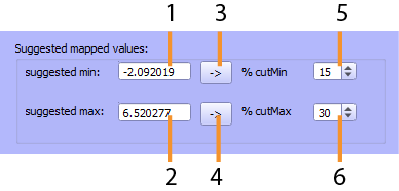
\includegraphics[scale=1]{images/14/volume_suggested_values2.png}
\caption{Volume rendering suggested mapped values. \textbf{1)} Suggested minimal value. \textbf{2)} Suggested maximal value. \textbf{3)} Apply suggested min value.  \textbf{4)} Apply suggested max value.\textbf{5)} Change the percentage of extreme minimal values to compute a new suggested minimal value. \textbf{6)} Change the percentage of extreme maximal values to compute a new suggested maximal value.}	
\label{volume_suggested_values}
 \end{figure}


\section{Extract isosurface from first selected volume}

\section{Flip or swap first selected volume}

\section{Change voxel size of first selected volume (keep dimensions, no resampling}

\section{Resample first selected volume (dimensions will be changed, and voxel size as well)}

\section{Reslice first selected volume}

\section{Median filter of first selected volume}

\section{Gaussian filter of first selected volume}

\section{Invert first selected volume}

